% =====================================================================
% paper_en.tex  --  ENGLISH VERSION (two columns)
% Build from docs: tectonic paper_en.tex, or run xelatex paper_en.tex twice.
% Font: Latin Modern (the classic LaTeX look) through fontspec.
% Placement rule: every table/figure/algorithm is placed right AFTER the paragraph
% that first mentions it, with [!htb]/[!t] (never [t] for in-column floats), so a
% float cannot jump ahead of the text that introduces it.
% =====================================================================
\documentclass[10pt,a4paper,twocolumn]{article}

\usepackage{fontspec}
\setmainfont{lmroman10-regular.otf}[BoldFont=lmroman10-bold.otf,ItalicFont=lmroman10-italic.otf,BoldItalicFont=lmroman10-bolditalic.otf]
\setsansfont{lmsans10-regular.otf}[BoldFont=lmsans10-bold.otf,ItalicFont=lmsans10-oblique.otf,BoldItalicFont=lmsans10-boldoblique.otf]
\setmonofont{lmmono10-regular.otf}[Scale=MatchLowercase,ItalicFont=lmmono10-italic.otf]

\usepackage{amsmath,amssymb}
\usepackage{graphicx}
\graphicspath{{../results/figures/}{results/figures/}}
\usepackage{booktabs}
\usepackage{array}
\newcolumntype{P}[1]{>{\raggedright\arraybackslash}p{#1}}
\usepackage{enumitem}
\usepackage{caption}
\usepackage{subcaption}
\usepackage{algorithm}
\usepackage{algpseudocode}
\usepackage{dblfloatfix}
\usepackage[a4paper,top=2.0cm,bottom=2.0cm,left=1.8cm,right=1.8cm,columnsep=0.7cm]{geometry}
\usepackage[hidelinks]{hyperref}
\usepackage{xurl}

% ---- Labels ----
\renewcommand{\algorithmicrequire}{\textbf{Input:}}
\renewcommand{\algorithmicensure}{\textbf{Output:}}

% ---- Layout ----
\setlength{\parindent}{1.2em}
\setlength{\parskip}{0pt}
\setlist{nosep,leftmargin=1.4em,itemsep=1pt,topsep=2pt}
\captionsetup{font=small,labelfont=bf,labelsep=period,skip=4pt}
\captionsetup[table]{skip=3pt}
\setlength{\textfloatsep}{8pt plus 2pt minus 2pt}
\setlength{\floatsep}{6pt plus 2pt minus 2pt}
\setlength{\intextsep}{6pt plus 2pt minus 2pt}
\setlength{\abovedisplayskip}{4pt}\setlength{\belowdisplayskip}{4pt}
\setlength{\tabcolsep}{3.5pt}
\renewcommand{\arraystretch}{1.08}
\emergencystretch=2em
\sloppy
\raggedbottom
\renewcommand{\topfraction}{0.9}\renewcommand{\bottomfraction}{0.85}
\renewcommand{\textfraction}{0.1}\renewcommand{\floatpagefraction}{0.8}
\renewcommand{\dbltopfraction}{0.9}\renewcommand{\dblfloatpagefraction}{0.8}

\newcommand{\sk}{\texttt{SGDRegressor}}
\newcommand{\x}{\times}
\newcommand{\mus}{\,\mu\mathrm{s}}
\newcommand{\supp}{\operatorname{supp}}
\newcommand{\relW}{\mathrm{Rel\_W}}
\newcommand{\relR}{\mathrm{Rel\_RMSE}}
\newcommand{\dridge}{d_{\mathrm{ridge}}}
\newcommand{\hd}[1]{\textbf{#1}\ }          % run-in heading

\title{\vspace{-0.8cm}\textbf{Scaled-Weight Decomposition for $L_2$-Regularized\\ Stochastic Gradient Descent on Sparse Data:\\ Verification and Reproduction in C++17}}
\author{Ngo Duy-Trang\\ Student ID 26125082 \\ \small Final project -- Introduction to Computer Science (CS161)}
\date{}

\begin{document}
\twocolumn[
  \begin{@twocolumnfalse}
    \maketitle
    \vspace{-1.2cm}
    \begin{center}
    \begin{minipage}{0.9\textwidth}
    \small
    \textbf{Abstract.}
    $L_2$ regularization forces every step of stochastic gradient descent (SGD) to update the whole weight vector, even though a sparse sample has very few nonzero entries, so the cost of a step grows with the number of dimensions.
    Splitting the weights into a scale factor and a vector can make this cost depend only on the number of nonzeros.
    This paper verifies the technique for least-squares regression by implementing SGD in plain C++ in two forms (direct update and scaled update) and comparing it with scikit-learn's \sk{} to answer two questions: (RQ1) how does the per-step cost change with the number of dimensions, the density and the number of samples; (RQ2) can the C++ version reproduce scikit-learn on real data.
    On synthetic sparse data with one million dimensions (20 nonzeros per sample), the scaled loop is more than 3000 times faster with the same held-out RMSE at the reported precision. On fully dense data the two loops are nearly equal.
    Each fitted model is evaluated for prediction time, RMSE, MAE and $R^2$ on the same held-out data for its configuration. On three house-price datasets, both C++ variants meet the numerical equivalence thresholds against scikit-learn at all five epoch budgets. The SGD weights approach Ridge while the best observed test RMSE occurs at different epoch budgets across datasets.
    All 7 hypotheses set by us are supported, although the results were measured on a single machine and a single compiler.
    Code and data are released for reproduction at \url{https://github.com/sitingfake/sgd-weight-splitting-cpp}.

    \smallskip
    \textbf{Keywords:} SGD, $L_2$ regularization, sparse data, Ridge regression, scikit-learn, C++17.
    \end{minipage}
    \end{center}
    \vspace{0.3cm}
  \end{@twocolumnfalse}
]

% =====================================================================
\section{Introduction}
Many machine-learning problems today have very high dimensionality, from hundreds of thousands to millions, yet the data are sparse: each sample has only a few nonzero features. Typical examples are natural-language processing (Bag-of-Words, TF-IDF~\cite{salton}), bioinformatics, graphs and recommender systems. At this scale, second-order methods and closed-form solutions based on matrix inversion are infeasible, because memory grows quadratically and time cubically with the dimension. Stochastic gradient descent (SGD)~\cite{robbins} therefore remains the main choice: it learns online, one sample at a time, with memory that grows only linearly with the dimension. To limit overfitting, $L_2$ regularization (Ridge)~\cite{hoerl}, which penalizes large weights, is added to the squared loss; the intercept is not penalized.

However, $L_2$ regularization creates a cost problem. Every update must shrink the whole weight vector, so the cost grows with the number of dimensions rather than with the number of nonzeros of the sample, even though the sample touches only a tiny part of the vector. The advantage of sparse data is thus lost exactly where it is needed most.

The remedy is known. Shalev-Shwartz et al.~\cite{pegasos} (Pegasos) and Bottou~\cite{bottou} proposed splitting the weight vector into the product of a scalar and a vector. The shrinkage then becomes a single multiplication of the scalar, the error term touches only the nonzero positions of the sample, and the cost of a step depends on the number of nonzeros instead of the dimension. scikit-learn's \sk{}~\cite{sklearn} is implemented in the same way. The technical details are given in Section~\ref{sec:method}.

Although the principle has been published, within the literature we surveyed two gaps remain. First, the foundational works experiment mainly with SVMs and the hinge loss, where many steps consist only of the shrinkage because the gradient is zero for samples outside the margin. With least-squares regression the residual is almost never zero, so every step also includes an update on the nonzero entries. This regime has not been compared systematically with the direct update across dimensions from one thousand to one million and densities from 0.1\% to 100\%. Second, scikit-learn has many internal details that affect numerical results, and we have not found a public comparison, with test code, showing that an independent C++17 implementation can match it step by step.

To fill these two gaps, we implement SGD in plain C++17 in two forms, direct update and scaled update, and compare it with scikit-learn's \sk{} to answer two research questions:
\begin{description}[leftmargin=1.9em,labelwidth=1.6em,labelsep=0.3em,itemsep=1pt]
\item[RQ1.] How does the per-step cost of the two forms change with the number of dimensions, the density and the number of samples?
\item[RQ2.] Can the C++ version reproduce \sk{} on real data?
\end{description}
For each configuration, we pair the timing measurements with held-out prediction quality for the same models and epoch budget.

% =====================================================================
\section{Data and Preprocessing}
To answer RQ1 we use synthetic sparse data: in real data, the dimension $n$, the density and the number of samples $m$ are usually tied together, whereas synthetic data let us vary one factor at a time through the three grids in Table~\ref{tab:grids}. Each sample has exactly $k$ distinct column indices chosen uniformly at random; the values are drawn from the standard normal distribution and then normalized to $\|x_i\|_2=1$ so that the gradient does not explode for large $n$. Labels are generated from a true weight vector drawn from the standard normal distribution, plus Gaussian noise with standard deviation 0.1. The generator uses the seed $[42,n,k,m]$, and each data file has a SHA-256 hash.

\begin{table}[!htb]
\centering\footnotesize
\caption{The three parameter grids of RQ1 ($\rho=k/n$ is the density).}\label{tab:grids}
\begin{tabular}{@{}P{0.7cm}P{4.2cm}P{2.9cm}@{}}
\toprule
Grid & Varied & Fixed\\
\midrule
A & $n\in\{10^3,10^4,10^5,10^6\}$ & $k=20$, $m=10^4$\\
B & $k\in\{5,50,500,2500,5000\}$, i.e.\ $\rho$ from 0.1\% to 100\% & $n=m=5000$\\
C & $m\in\{10^3,10^4,10^5,10^6\}$ & $n=10^4$, $k=20$\\
\bottomrule
\end{tabular}
\end{table}

For each synthetic configuration, $m$ is the training size. The held-out set contains $m/5$ rows generated with the same true weights and a separate stream, seeded with $[42,n,k,m,1]$, for its features and noise. Direct, Scaled and \sk{} share both sets.

To answer RQ2 we use three public house-price datasets, ranging from small ($m\approx400$) to medium ($m\approx20{,}000$) (Table~\ref{tab:real}). All three have few features and are processed as dense arrays in scikit-learn. Taiwan~\cite{yeh} contains transactions in Xindian District with 6 features (transaction date, house age, distance to the MRT station, number of convenience stores, latitude, longitude); the column \texttt{No} is dropped. California~\cite{pace} comes from the 1990 census with 8 features; the target is artificially capped, with about 4.7\% of the observations at the ceiling. King County~\cite{openml} contains transactions from May 2014 to May 2015 with 17 numeric features, dropping \texttt{id}, \texttt{date} and \texttt{zipcode} (a categorical identifier with very many levels); prices are strongly right-skewed (median 450,000 USD, maximum 7,700,000 USD).

\begin{table}[!htb]
\centering\footnotesize
\caption{The real datasets of RQ2.}\label{tab:real}
\begin{tabular}{@{}lrrr@{}}
\toprule
Dataset & $m$ & $n$ & Train/Test\\
\midrule
Taiwan (UCI 477) & 414 & 6 & 331/83\\
California Housing & 20,640 & 8 & 16,512/4128\\
King County (OpenML 42092) & 21,613 & 17 & 17,290/4323\\
\bottomrule
\end{tabular}
\end{table}

The data are split 80/20 with \texttt{random\_state=42}, \texttt{shuffle=True}; the row indices are saved so that C++, scikit-learn and Ridge share one partition. Z-score standardization is applied to both $X$ and $y$, with the mean and standard deviation ($\mathrm{ddof}=0$) computed on the training set only, to avoid data leakage. For evaluation, predictions are transformed back to the original units before computing RMSE, MAE and $R^2$. The data are written in the binary format \texttt{SGDCSR01} (the first 32 bytes hold the identifier string, $m$, $n$ and nnz; then \texttt{indptr} and \texttt{indices} as int32, \texttt{data} and $y$ as float64), which avoids parsing CSV text and preserves every bit of float64 between Python and C++.

The RQ2 runner checks that the CSR training values and their row order match the dense training arrays. Both benchmark runners record SHA-256 identifiers for the shared training and test inputs.

% =====================================================================
\section{Method}\label{sec:method}
The objective is
\begin{equation}
J(w,b)=\frac1m\sum_{i=1}^{m}\tfrac12\bigl(w^\top x_i+b-y_i\bigr)^2+\frac{\alpha}{2}\|w\|_2^2,
\label{eq:J}
\end{equation}
where the intercept $b$ is not penalized. For standardized data, the closed-form Ridge solution~\cite{hoerl} is $\hat w_{\mathrm{ridge}}=(X^\top X+\alpha_{\mathrm{ridge}}I)^{-1}X^\top y$. Since scikit-learn's \texttt{Ridge} minimizes $\|Xw-y\|_2^2+\alpha_{\mathrm{ridge}}\|w\|_2^2$ (not divided by $m$), multiplying \eqref{eq:J} by $2m$ shows that the two objectives coincide when
\begin{equation}
\alpha_{\mathrm{ridge}}=m_{\mathrm{train}}\cdot\alpha_{\mathrm{sgd}}.
\label{eq:alpha}
\end{equation}
Then $\hat w_{\mathrm{ridge}}$ is the point that SGD approaches as the number of epochs $E\to\infty$.

At step $t$ on sample $(x_i,y_i)$, with learning rate $\eta_t=\eta_0/t^{\texttt{power\_t}}$ (the \texttt{invscaling} schedule), direct SGD (Algorithm~\ref{alg:direct}) updates
\begin{equation}
w_{t+1}=(1-\eta_t\alpha)\,w_t-\eta_t(\hat y_i-y_i)\,x_i.
\label{eq:upd}
\end{equation}
Shrinking the whole $w$ (the shrinkage factor is clipped from below at 0) is the $O(n)$ bottleneck, whereas the gradient is added at only $k\ll n$ nonzero positions.

\begin{algorithm}[!htb]
\caption{Direct SGD}\label{alg:direct}
\small
\begin{algorithmic}[1]
\Require CSR $X$, $y$, $E$, $\alpha$, $\eta_0$, \texttt{power\_t}, $\gamma$ (intercept\_decay)
\State $w\gets 0,\ b\gets0,\ t\gets1$
\For{each epoch, each sample $i$ in order}
  \State $p\gets b+\sum_{j\in\supp(x_i)}w_jx_{ij}$
  \State $g\gets\mathrm{clip}(p-y_i,\pm10^{12})$
  \State $\eta\gets\eta_0/t^{\texttt{power\_t}}$
  \State $w_j\gets\max(0,1-\eta\alpha)\,w_j$ \textbf{for all} $j=1..n$ \Comment{$O(n)$}
  \State $u\gets-\eta g$
  \If{$u\neq0$}
    \State $w_j\gets w_j+u\,x_{ij}$, $j\in\supp(x_i)$ \Comment{$O(k)$}
    \State $b\gets b+\gamma u$
  \EndIf
  \State $t\gets t+1$
\EndFor
\State \Return $w,b$
\end{algorithmic}
\end{algorithm}

Scaled SGD (Algorithm~\ref{alg:scaled}) sets $w=s\cdot v$ with $s_1=1$, $v_1=0$. The shrinkage becomes just $s\leftarrow\max(0,1-\eta_t\alpha)\,s$, costing $O(1)$, and the error term touches only $k$ positions of $v$:
\begin{equation}
v_j\leftarrow v_j+\frac{u_t}{s}\,x_{ij},\quad j\in\supp(x_i),\qquad u_t=-\eta_t(\hat y_i-y_i),
\label{eq:sv}
\end{equation}
where $s$ is the value after shrinking. The prediction is computed indirectly as $\hat y=s\,(v^\top x_i)+b$. The cost of a step drops from $O(n)$ to $O(k)$, and the sequence of iterates is unchanged in exact arithmetic, because $s_{t+1}v_{t+1}=(1-\eta_t\alpha)\,w_t+u_tx_i$. When $s$ becomes too small, the division by $s$ makes $v$ blow up, so we renormalize $v\leftarrow s\,v,\ s\leftarrow1$ when $s<10^{-9}$. This step costs $O(n)$ but is rare: with $\alpha=10^{-4}$ and $\eta_0=0.01$, about $4\x10^{9}$ steps are needed for $s$ to reach the threshold. In the largest experiment ($3\x10^6$ steps), $s\approx0.91$ and the number of resets is 0, so this cost has no effect. The reset branch is tested separately with a forced configuration $\alpha=10$.

\begin{algorithm}[!htb]
\caption{Scaled SGD, $w=s\cdot v$}\label{alg:scaled}
\small
\begin{algorithmic}[1]
\Require as in Algorithm~\ref{alg:direct}
\State $v\gets0,\ s\gets1,\ b\gets0,\ t\gets1$
\For{each epoch, each sample $i$ in order}
  \State $p\gets s\sum_{j\in\supp(x_i)}v_jx_{ij}+b$
  \State $g\gets\mathrm{clip}(p-y_i,\pm10^{12})$
  \State $\eta\gets\eta_0/t^{\texttt{power\_t}}$
  \State $s\gets\max(0,1-\eta\alpha)\,s$ \Comment{$O(1)$}
  \If{$s<10^{-9}$}
    \State $v\gets s\,v,\ s\gets1$ \Comment{$O(n)$, rare}
  \EndIf
  \State $u\gets-\eta g$
  \If{$u\neq0$}
    \State $v_j\gets v_j+(u/s)\,x_{ij}$, $j\in\supp(x_i)$ \Comment{$O(k)$}
    \State $b\gets b+\gamma u$
  \EndIf
  \State $t\gets t+1$
\EndFor
\State \Return $w=s\cdot v,\ b$ \Comment{outside the timed loop}
\end{algorithmic}
\end{algorithm}

The C++ version follows scikit-learn 1.9.1's Cython code in these respects: the $(s,v)$ representation as \texttt{wscale}/\texttt{w}; the reset threshold $10^{-9}$; the execution order \emph{dot} $\to$ gradient clipping $\to$ shrinkage $\to$ add (the add happens only when $u\neq0$); gradient clipping at $\pm10^{12}$; $b$ is not shrunk and uses \texttt{intercept\_decay}; the \texttt{invscaling} schedule with $t$ starting at 1 and continuing across epochs; sequential traversal when \texttt{shuffle=False}; no early stopping (\texttt{tol=None}).

For RQ1 we use the squared loss, $\alpha=10^{-4}$, \texttt{fit\_intercept=False}, \texttt{invscaling} with $\eta_0=0.01$, $\texttt{power\_t}=0.25$, $E=3$, $w_0=0$. On Grid A we compute the log-log slope of $T$ between $n=10^4$ and $n=10^6$ (expected $\beta_{\mathrm{direct}}\approx1$, $\beta_{\mathrm{scaled}}\approx0$). For RQ2 we set \texttt{fit\_intercept=True} (\texttt{intercept\_decay=1}), keep $\alpha$ and the schedule, and retrain from scratch with $E\in\{1,5,20,100,500\}$ for Direct, Scaled and \sk{}. The Ridge reference uses a Cholesky fit with no epoch budget. Besides RMSE, MAE and $R^2$ on the test set (original units), we measure three relative errors: $\relW$ between $w_{\mathrm{cpp}}$ and $w_{\mathrm{sk}}$, $\dridge(E)$ between $w(E)$ and $\hat w_{\mathrm{ridge}}$, both of the form $\|a-b\|_2/\|b\|_2$, and $\relR=|\mathrm{RMSE}_{\mathrm{cpp}}-\mathrm{RMSE}_{\mathrm{sk}}|/\mathrm{RMSE}_{\mathrm{sk}}$. We set seven hypotheses, with quantitative criteria in Table~\ref{tab:hyp}: H1-a (speed-up for large $n$), H1-b (log-log slope), H1-c (dense data), H1-d (invariance to $m$), H1-e (Direct $\equiv$ Scaled), H2-a (C++ $\equiv$ scikit-learn), H2-b (same trajectory toward Ridge).

The revised measurements used Windows 11, MinGW-W64 GCC 14.2.0 (\texttt{-std=c++17 -O2 -static}), Python 3.12.14, NumPy 2.5.4, SciPy 1.18.1 and scikit-learn 1.9.1. The code runs single-threaded by setting \texttt{OMP\_NUM\_THREADS}, \texttt{OPENBLAS\_NUM\_THREADS} and \texttt{MKL\_NUM\_THREADS} to 1. Each measurement consists of 1 warm-up run and 7 repeats, and we report the median and the IQR.

\hd{Training time.} The full fit timer covers the C++ training call through the final weight vector or the scikit-learn \texttt{fit} call, including its input validation. Data loading, preprocessing and process startup are outside this interval. C++ additionally records the SGD loop using \texttt{std::chrono::steady\_clock}. In RQ1, the loop median divided by $mE$ defines the per-update cost for Direct and Scaled. The scikit-learn reference column divides the full fit median by $mE$.

\hd{Held-out prediction.} For each method, the first timed fit supplies $w$ and $b$. A shared Python routine times $Xw+b$ across the entire test set and, for RQ2, transforms the predictions back to the original units. RMSE, MAE and $R^2$ use the first timed prediction and are calculated after the timer stops.

% =====================================================================
\section{Results and Discussion}
\hd{RQ1: per-step cost.} Costs are in $\mu$s per update (median). The C++ loop speed-up is $T_{\mathrm{direct}}/T_{\mathrm{scaled}}$. On all three grids, the weights of Direct and Scaled differ by a relative error of at most $5.11\x10^{-14}$, i.e.\ at the float64 rounding level (H1-e).

\hd{Dimension (Grid A, Table~\ref{tab:A}, Figure~\ref{fig:A}).} The cost of Direct grows with $n$ with slope $\beta_{\mathrm{direct}}=1.002$, consistent with $O(n)$. The cost of Scaled is almost flat ($\approx0.036$--$0.037\mus$ from $n=10^3$ to $10^5$), with $\beta_{\mathrm{scaled}}=0.133$. At $n=10^6$ the loop speed-up reaches $3197.90\x$. The cost of Scaled rises to $0.0688\mus$ at $n=10^6$; a plausible explanation is that the array $v$ (8 MB) exceeds the L2 cache (not confirmed with hardware counters). The full fit medians at this point are 6598.362 ms for Direct and 4.367 ms for Scaled.

\begin{table}[!htb]
\centering\small
\caption{Grid A ($k=20$, $m=10^4$): C++ loop and sklearn fit in $\mu$s per update.}\label{tab:A}
\begin{tabular}{@{}rrrrr@{}}
\toprule
$n$ & Direct & Scaled & sklearn & Speed-up\\
\midrule
$10^3$ & 0.2503 & 0.0362 & 0.0819 & $6.91\x$\\
$10^4$ & 2.1828 & 0.0372 & 0.0740 & $58.65\x$\\
$10^5$ & 21.9501 & 0.0365 & 0.0870 & $600.71\x$\\
$10^6$ & 219.9087 & 0.0688 & 0.1499 & $\mathbf{3197.90\x}$\\
\bottomrule
\end{tabular}
\end{table}

\begin{figure}[!htb]
\centering
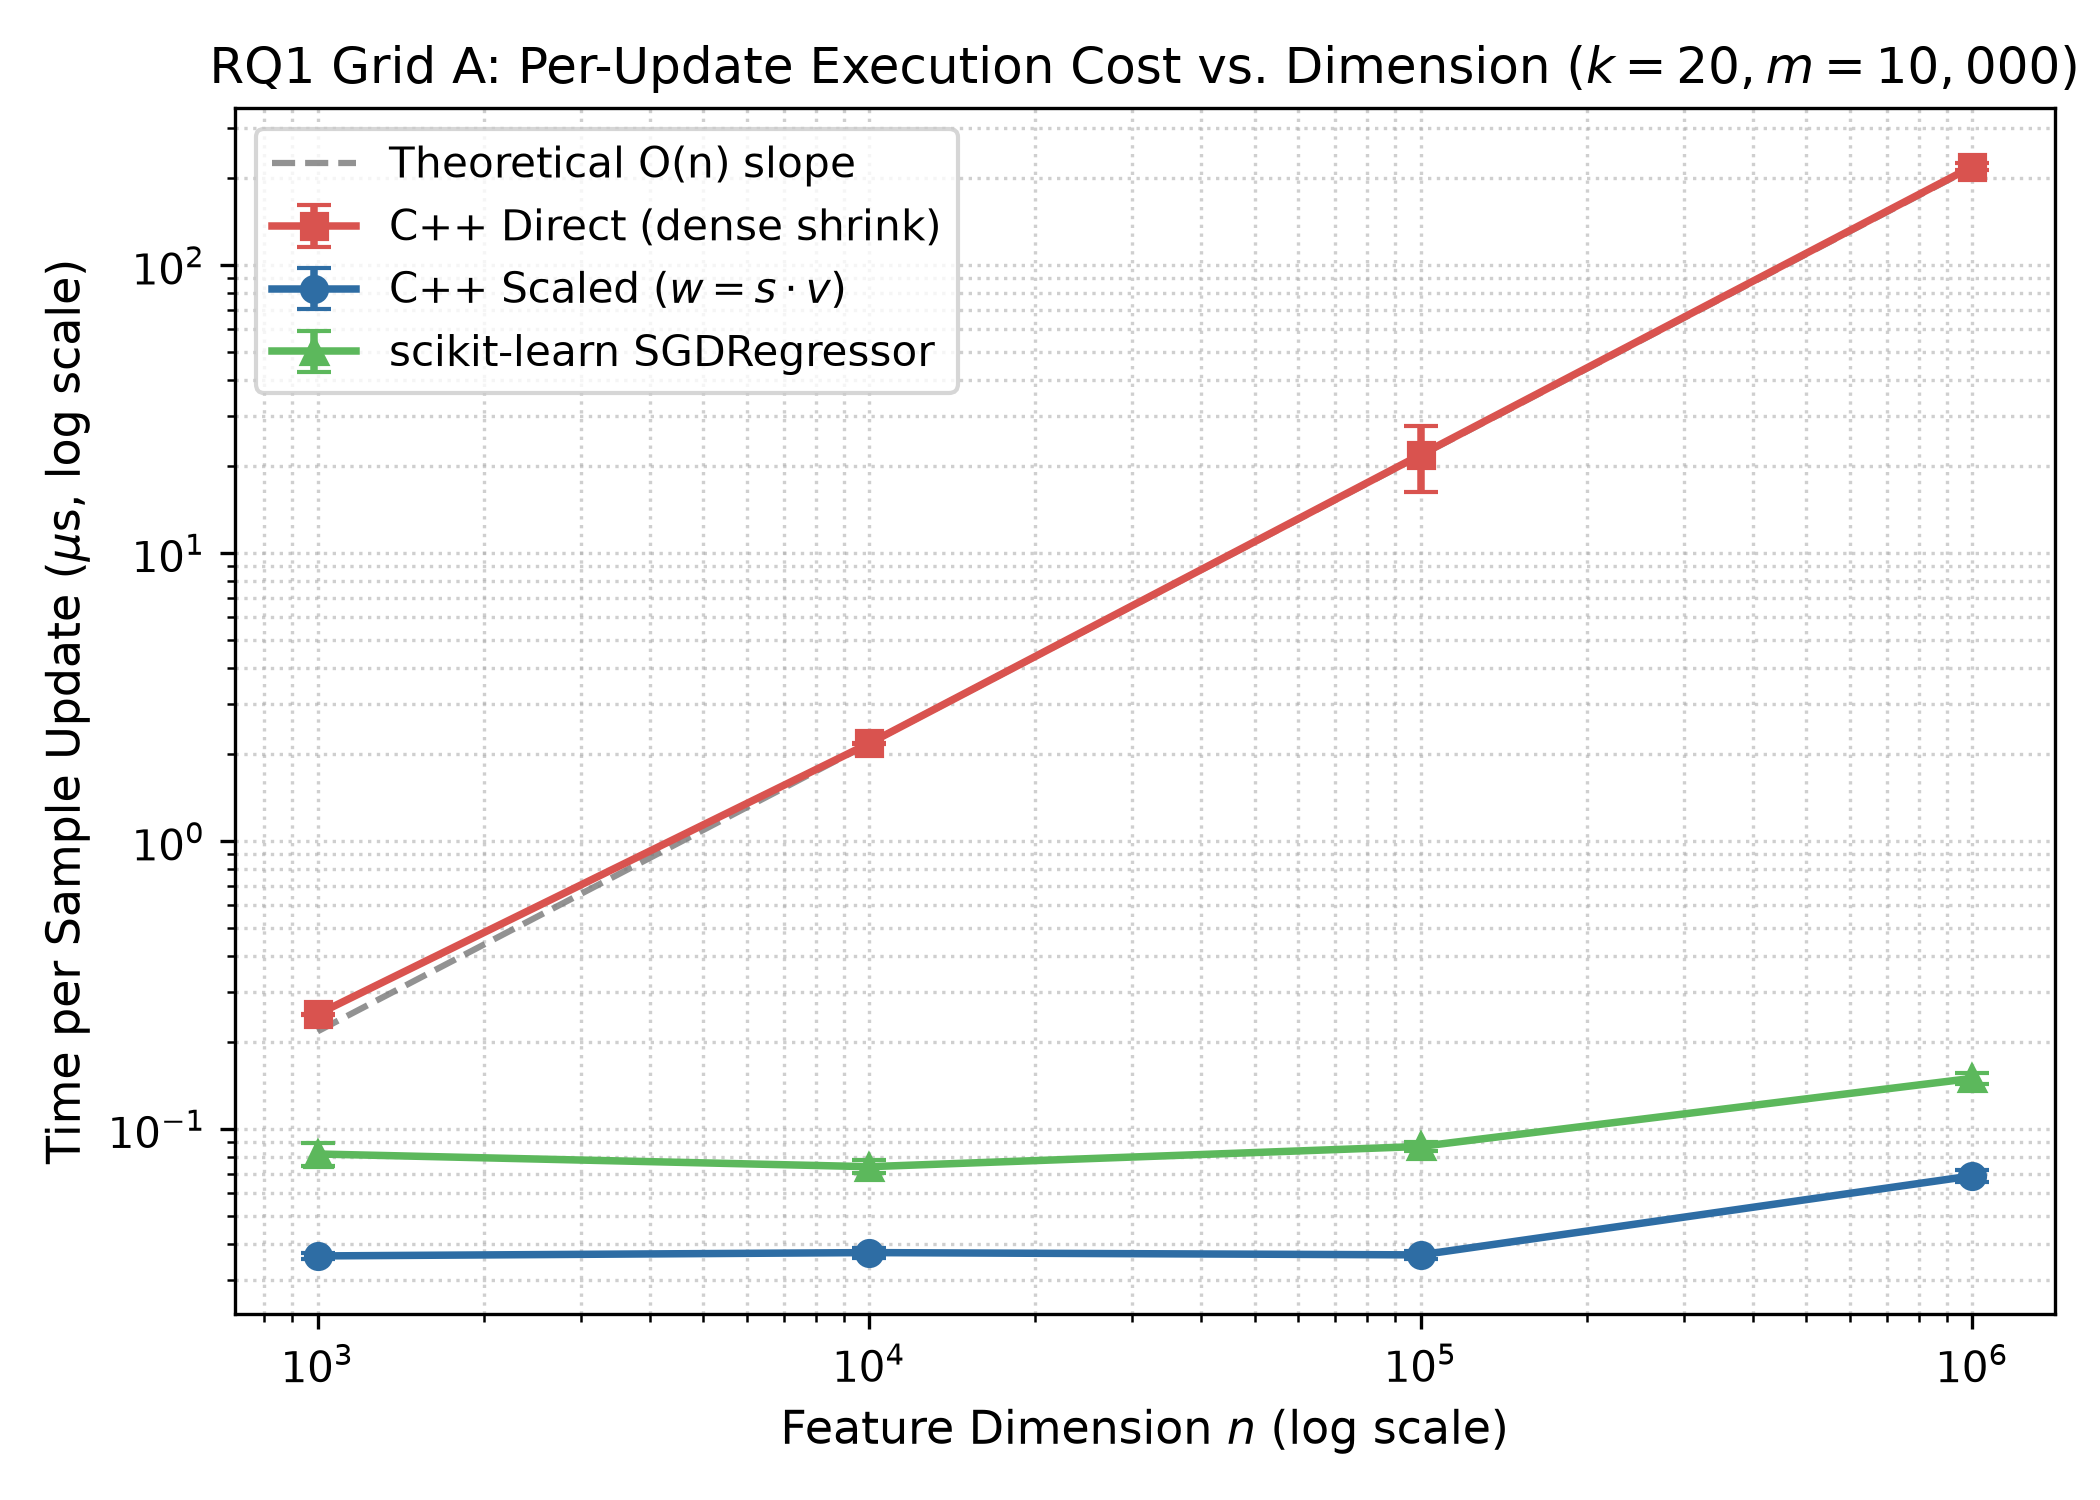
\includegraphics[width=\columnwidth]{fig1_rq1_gridA_dim.png}
\caption{Grid A: per-update cost versus dimension $n$ (log-log, $k=20$, $m=10^4$). Dashed line: theoretical $O(n)$ slope.}\label{fig:A}
\end{figure}

\hd{Density (Grid B, Table~\ref{tab:B}, Figure~\ref{fig:B}).} The advantage shrinks as the density $\rho$ grows: $57.15\x$ at 0.1\%, $19.94\x$ at 1\%, $2.95\x$ at 10\%, and $1.12\x$ at 100\%. At 100\% density the two forms have the same order $O(n)$. The measured improvement is modest (Figure~\ref{fig:B}).

\begin{table}[!htb]
\centering\small
\caption{Grid B ($n=m=5000$): C++ loop and sklearn fit in $\mu$s per update.}\label{tab:B}
\begin{tabular}{@{}rrrrrr@{}}
\toprule
$k$ & $\rho$ & Direct & Scaled & sklearn & Speed-up\\
\midrule
5 & 0.1\% & 1.0782 & 0.0189 & 0.0845 & $57.15\x$\\
50 & 1\% & 1.1085 & 0.0556 & 0.1460 & $19.94\x$\\
500 & 10\% & 1.6189 & 0.5488 & 0.8234 & $2.95\x$\\
2500 & 50\% & 3.8654 & 3.5937 & 3.9898 & $1.08\x$\\
5000 & 100\% & 6.5719 & 5.8886 & 8.3433 & $1.12\x$\\
\bottomrule
\end{tabular}
\end{table}

\begin{figure}[!htb]
\centering
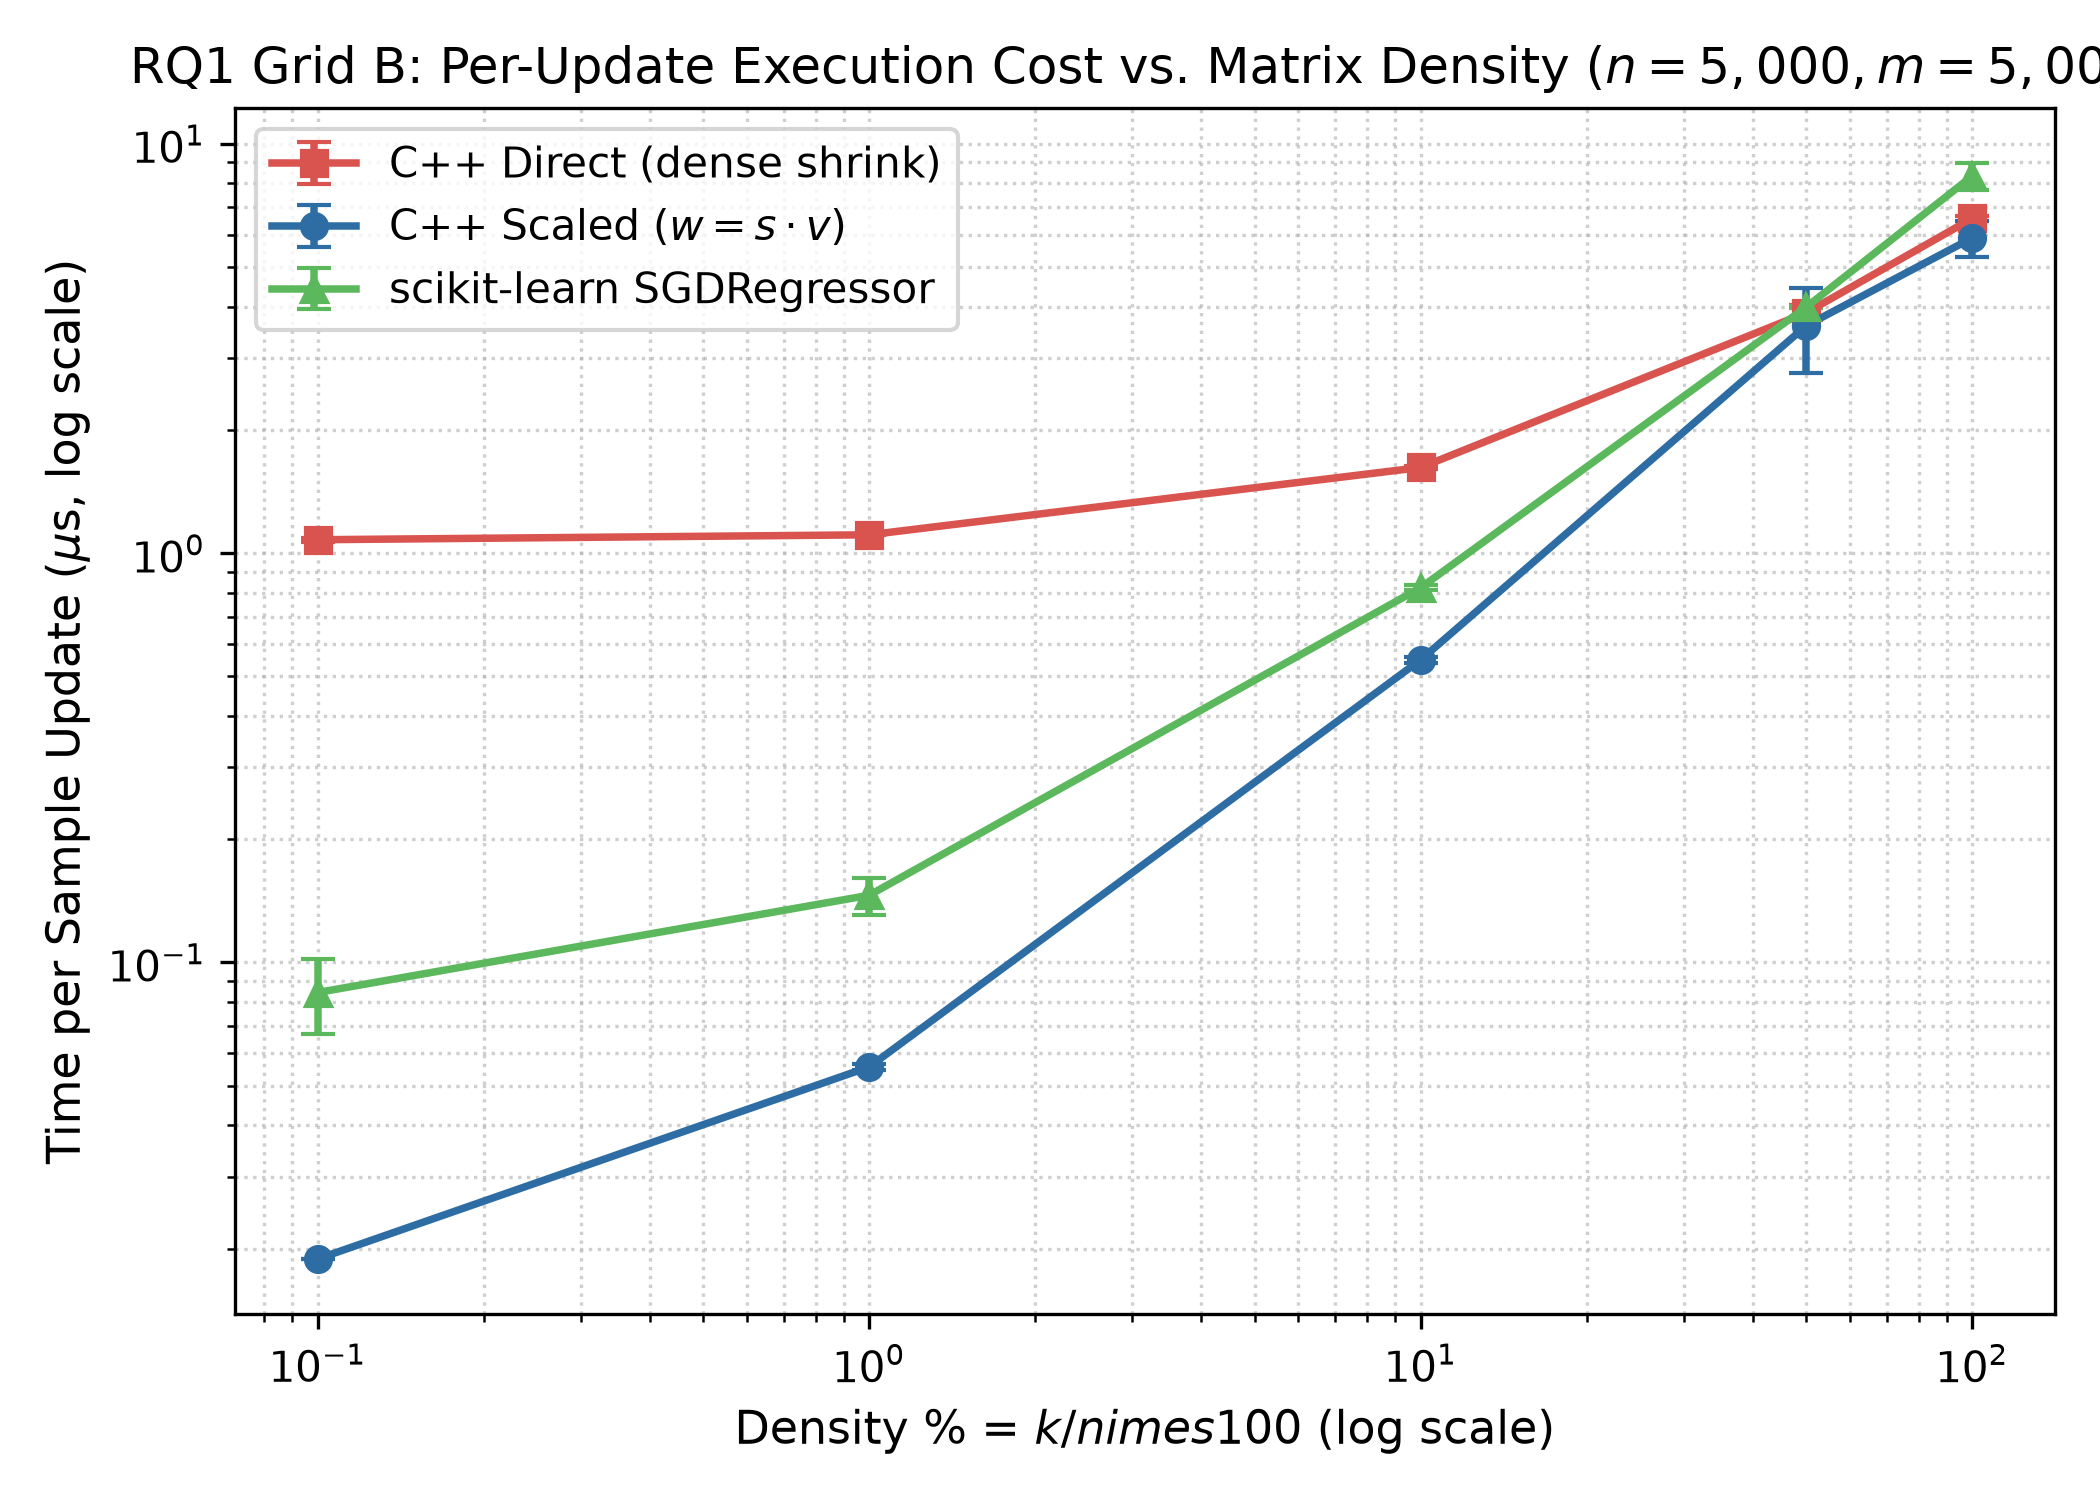
\includegraphics[width=\columnwidth]{fig2_rq1_gridB_density.png}
\caption{Grid B: per-update cost versus density $k/n$ ($n=m=5000$). Error bars show the spread across repeated runs.}\label{fig:B}
\end{figure}

\hd{Sample count (Grid C, Figure~\ref{fig:C}).} As $m$ grows from $10^3$ to $10^6$, the cost of Scaled varies only within $0.0346$--$0.0384\mus$ (max/min ratio 1.11), and the speed-up stays between $56.75\x$ and $62.30\x$ (H1-d).

\begin{figure}[!htb]
\centering
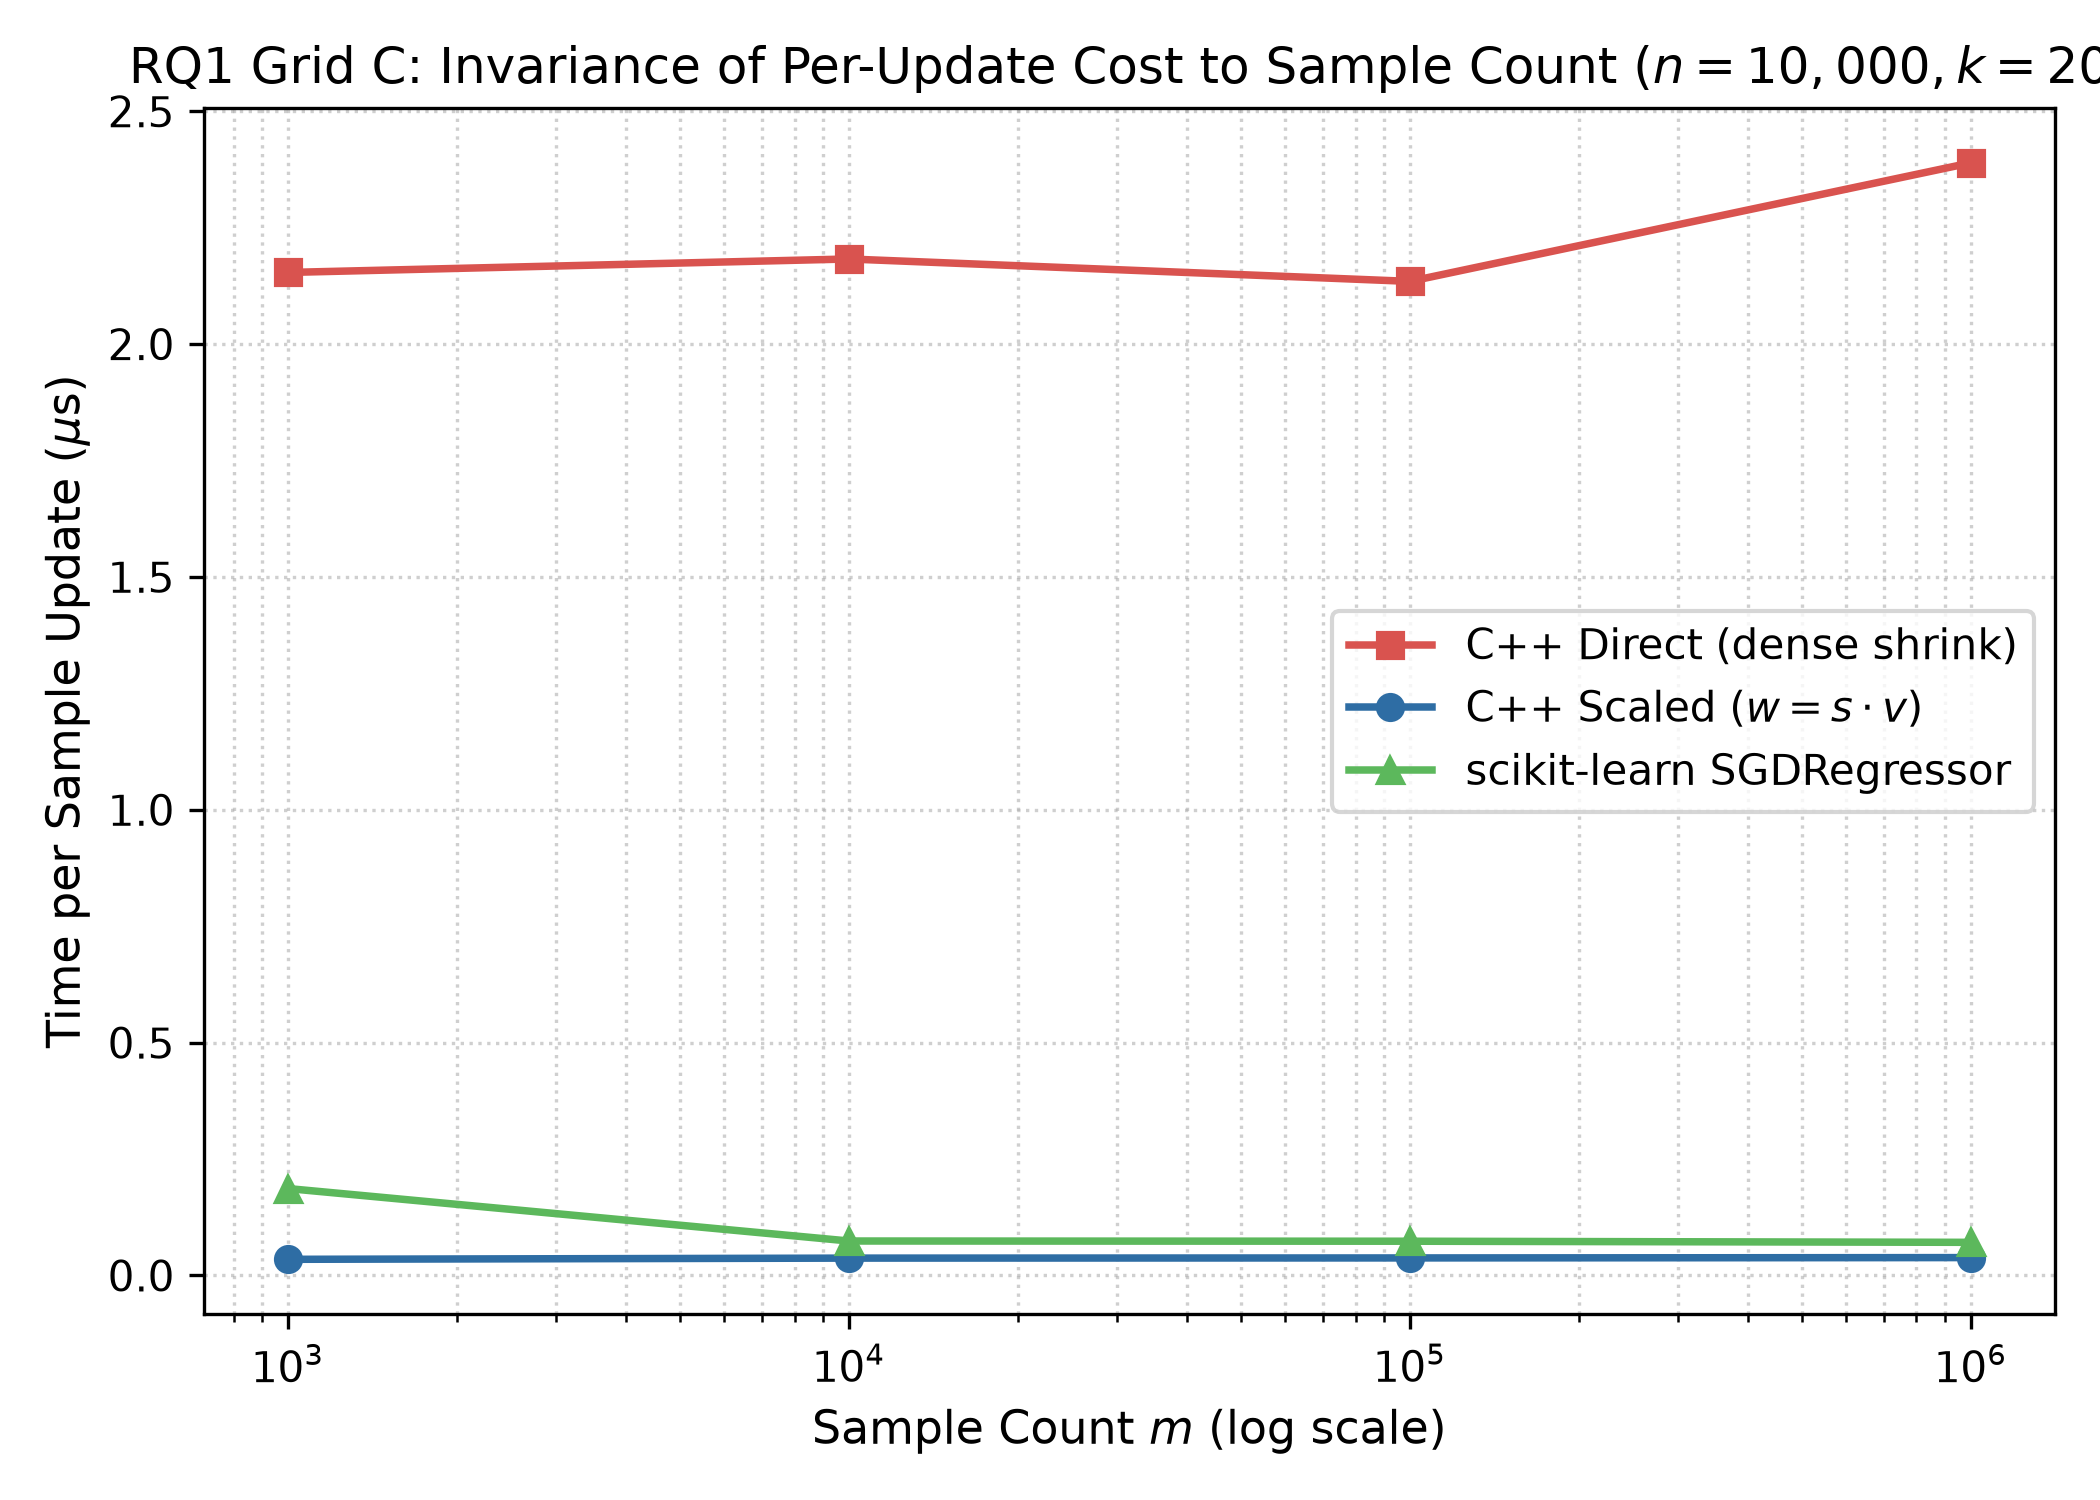
\includegraphics[width=\columnwidth]{fig3_rq1_gridC_samples.png}
\caption{Grid C: per-update cost versus number of samples $m$ ($n=10^4$, $k=20$).}\label{fig:C}
\end{figure}

\hd{Paired results on synthetic data.} Table~\ref{tab:paired-rq1} reports full fit time together with prediction time and error for two ends of the sparsity range. All three methods agree on the test metrics to the displayed precision in both configurations. On the million-feature configuration, the full-fit Direct/Scaled ratio is about $1511\x$, since full fit includes allocation and reconstruction of the final weights. The near-zero test $R^2$ there reflects the prediction quality after the fixed three-epoch budget.

\begin{table}[!htb]
\centering\footnotesize
\setlength{\tabcolsep}{2.4pt}
\caption{RQ1 paired fit and test results after 3 epochs. Time columns show medians for full fit and prediction on the entire held-out set.}\label{tab:paired-rq1}
\begin{tabular}{@{}lrrrrr@{}}
\toprule
Model & Fit (ms) & Test ($\mu$s) & RMSE & MAE & $R^2$\\
\midrule
\multicolumn{6}{@{}l}{\textit{$n=10^6$, $k=20$ (2,000 test rows)}}\\
C++ Direct & 6,598.362 & 42.4 & 1.01252 & 0.80657 & -0.00089\\
C++ Scaled & 4.367 & 51.4 & 1.01252 & 0.80657 & -0.00089\\
scikit-learn & 4.498 & 49.3 & 1.01252 & 0.80657 & -0.00089\\
\addlinespace[2pt]
\multicolumn{6}{@{}l}{\textit{$n=k=5000$ (1,000 test rows)}}\\
C++ Direct & 98.581 & 4,116.2 & 1.00081 & 0.80595 & 0.00417\\
C++ Scaled & 88.339 & 4,135.5 & 1.00081 & 0.80595 & 0.00417\\
scikit-learn & 125.149 & 3,941.6 & 1.00081 & 0.80595 & 0.00417\\
\bottomrule
\end{tabular}
\end{table}

\hd{RQ2: equivalence and convergence.} Both C++ variants meet the equivalence thresholds against \sk{} at all 15 dataset and epoch combinations (3 datasets $\x$ 5 values of $E$). For Scaled, every measured deviation ($\relW$, $\relR$, MAE and $R^2$) is zero in this environment. For Direct, the largest $\relW$ and $\relR$ are $2.49\x10^{-14}$ and $9.32\x10^{-16}$. At every epoch, $|d_{\mathrm{scaled}}-d_{\mathrm{sk}}|/d_{\mathrm{sk}}=0$, so these two models follow the same trajectory toward the Ridge solution (H2-b). The distance $\dridge$ decreases monotonically with $E$ on all three datasets (Table~\ref{tab:conv}, Figure~\ref{fig:conv}), but with \texttt{invscaling}, SGD has not reached the Ridge solution after 500 epochs: 0.71\% remains for Taiwan, 1.55\% for California and 4.99\% for King County. The test RMSE at $E=500$ is very close to Ridge on Taiwan (7.3187 vs.\ 7.3146) and California (0.7444 vs.\ 0.7455); on King County it differs by about 0.5\% (215,620 vs.\ 214,473 USD). The RMSE, MAE and $R^2$ curves versus epochs are in the Appendix.

\hd{Paired results on housing data.} At $E=100$, Scaled reduces median fit time relative to Direct by about 11\% on Taiwan, 11\% on California and 4\% on King County, with the same test scores at the displayed precision (Table~\ref{tab:paired-rq2}). The California fit IQR is 1.102 ms for Direct and 0.724 ms for Scaled. Figure~\ref{fig:fit-rmse} shows the measured fit time and test RMSE for each model and epoch budget. The lowest observed SGD test RMSE occurs at $E=5$ for Taiwan, $E=20$ for California and $E=1$ for King County. For example, the California Scaled fit takes 9.096 ms at $E=20$ with RMSE 0.7404. At $E=500$, it takes 228.331 ms and is closer to Ridge, with test RMSE 0.7444. The complete tables, with timing IQRs and all three test metrics, are in \texttt{results/tables/}.


\begin{figure*}[!t]
\centering
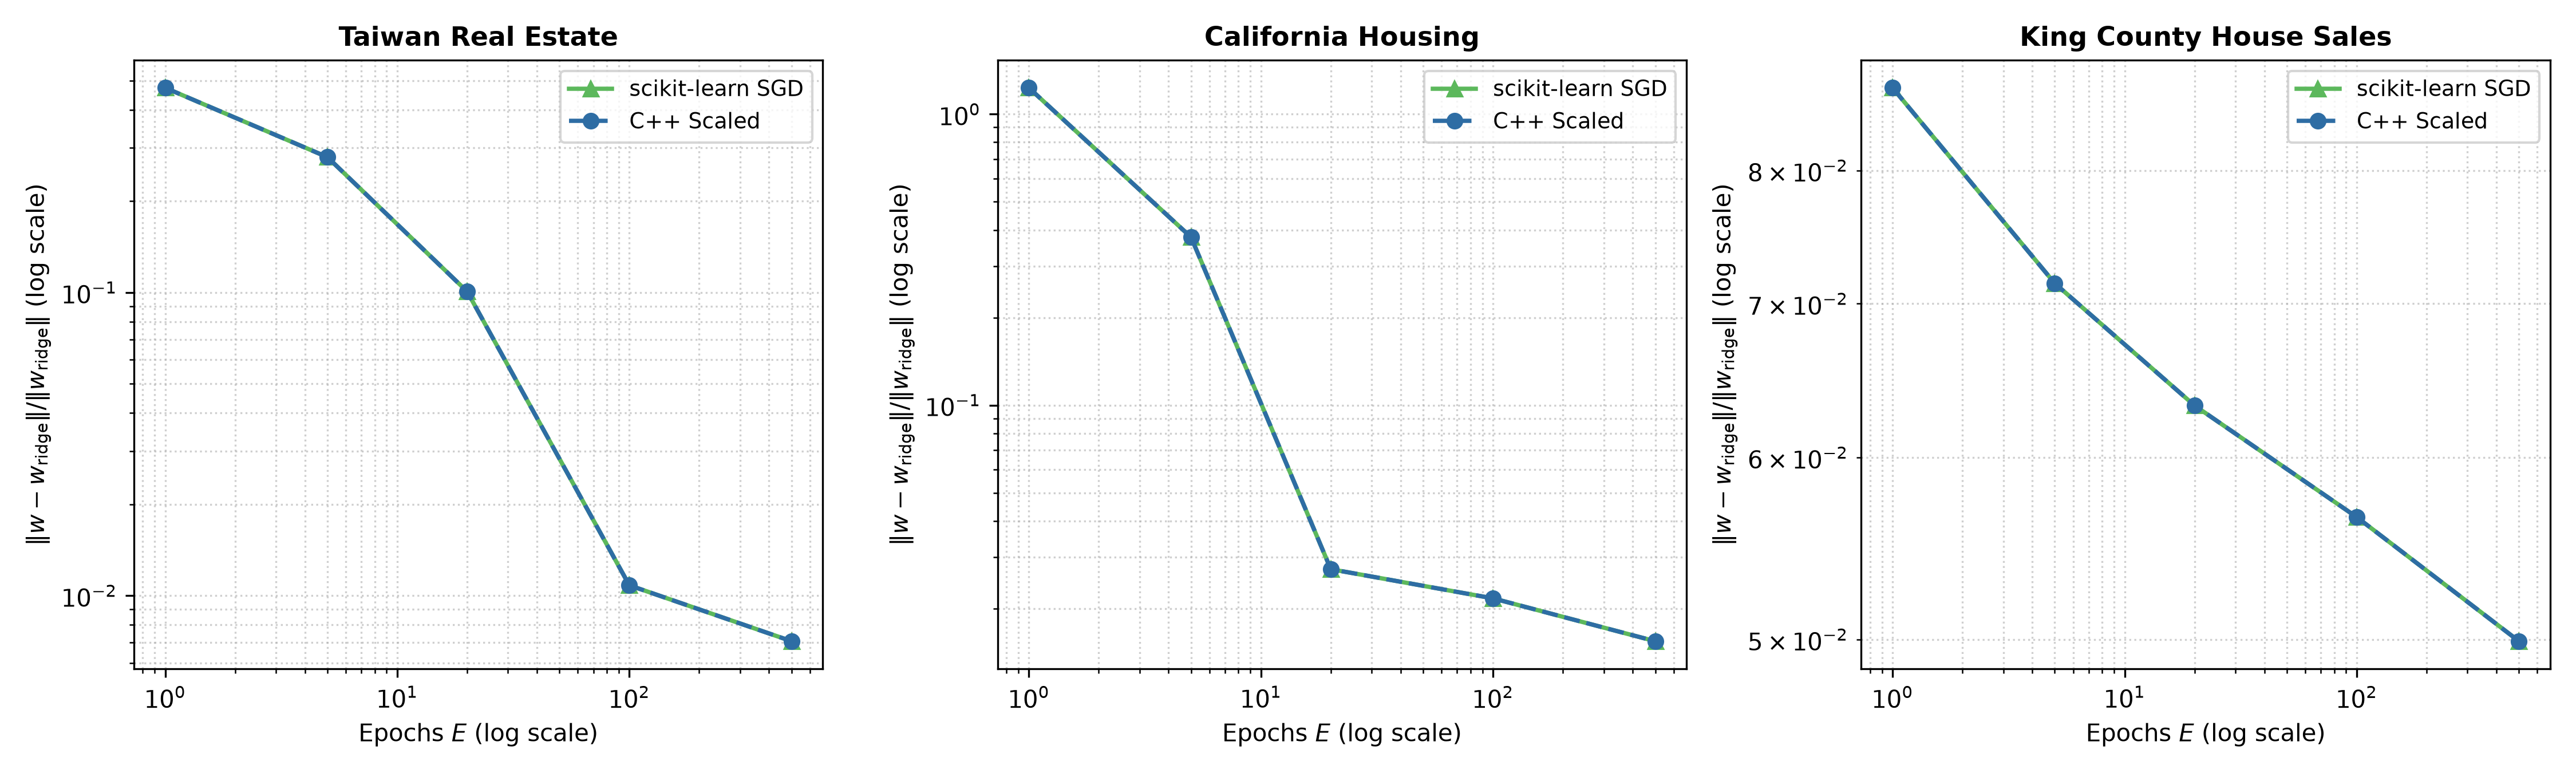
\includegraphics[width=0.92\textwidth]{figS1_rq2_convergence.png}
\caption{Relative distance to the Ridge solution versus number of epochs $E$ (log-log). The curves of scikit-learn and C++ Scaled coincide.}\label{fig:conv}
\end{figure*}

\begin{table}[!htb]
\centering\small
\caption{Relative distance to the Ridge solution $\dridge(E)$, and quality at $E=500$ (C++ Scaled and scikit-learn give identical values). RMSE in original units: Taiwan 10,000 NTD/Ping, California 100,000 USD, King County USD.}\label{tab:conv}
\begin{tabular}{@{}lrrr@{}}
\toprule
 & Taiwan & California & King County\\
\midrule
$\dridge(E{=}1)$ & 0.4735 & 1.2310 & 0.0869\\
$\dridge(E{=}5)$ & 0.2796 & 0.3775 & 0.0714\\
$\dridge(E{=}20)$ & 0.1008 & 0.0273 & 0.0632\\
$\dridge(E{=}100)$ & 0.0108 & 0.0217 & 0.0565\\
$\dridge(E{=}500)$ & 0.0071 & 0.0155 & 0.0499\\
\midrule
RMSE, Ridge & 7.3146 & 0.7455 & 214,473.46\\
RMSE, SGD ($E{=}500$) & 7.3187 & 0.7444 & 215,619.85\\
$R^2$, Ridge & 0.6811 & 0.5758 & 0.6957\\
$R^2$, SGD ($E{=}500$) & 0.6807 & 0.5771 & 0.6925\\
\bottomrule
\end{tabular}
\end{table}

\begin{table}[!htb]
\centering\footnotesize
\setlength{\tabcolsep}{2.4pt}
\caption{RQ2 paired fit and test results for SGD at 100 epochs and the Ridge fit. Time columns show medians for full fit and prediction on the entire held-out set. RMSE and MAE use the units of Table~\ref{tab:conv}.}\label{tab:paired-rq2}
\begin{tabular}{@{}lrrrrr@{}}
\toprule
Model & Fit (ms) & Test ($\mu$s) & RMSE & MAE & $R^2$\\
\midrule
\multicolumn{6}{@{}l}{\textit{Taiwan}}\\
C++ Direct & 0.856 & 4.9 & 7.3201 & 5.3156 & 0.6806\\
C++ Scaled & 0.758 & 4.6 & 7.3201 & 5.3156 & 0.6806\\
scikit-learn & 2.800 & 5.4 & 7.3201 & 5.3156 & 0.6806\\
Ridge & 0.324 & 4.5 & 7.3146 & 5.3053 & 0.6811\\
\addlinespace[2pt]
\multicolumn{6}{@{}l}{\textit{California}}\\
C++ Direct & 51.543 & 15.9 & 0.7424 & 0.5348 & 0.5794\\
C++ Scaled & 45.702 & 19.1 & 0.7424 & 0.5348 & 0.5794\\
scikit-learn & 82.356 & 12.2 & 0.7424 & 0.5348 & 0.5794\\
Ridge & 1.235 & 12.5 & 0.7455 & 0.5332 & 0.5758\\
\addlinespace[2pt]
\multicolumn{6}{@{}l}{\textit{King County}}\\
C++ Direct & 63.711 & 23.5 & 215,620.04 & 125,059.64 & 0.6925\\
C++ Scaled & 61.036 & 26.3 & 215,620.04 & 125,059.64 & 0.6925\\
scikit-learn & 105.055 & 18.1 & 215,620.04 & 125,059.64 & 0.6925\\
Ridge & 1.354 & 16.2 & 214,473.46 & 128,154.42 & 0.6957\\
\bottomrule
\end{tabular}
\end{table}

\begin{figure*}[!t]
\centering
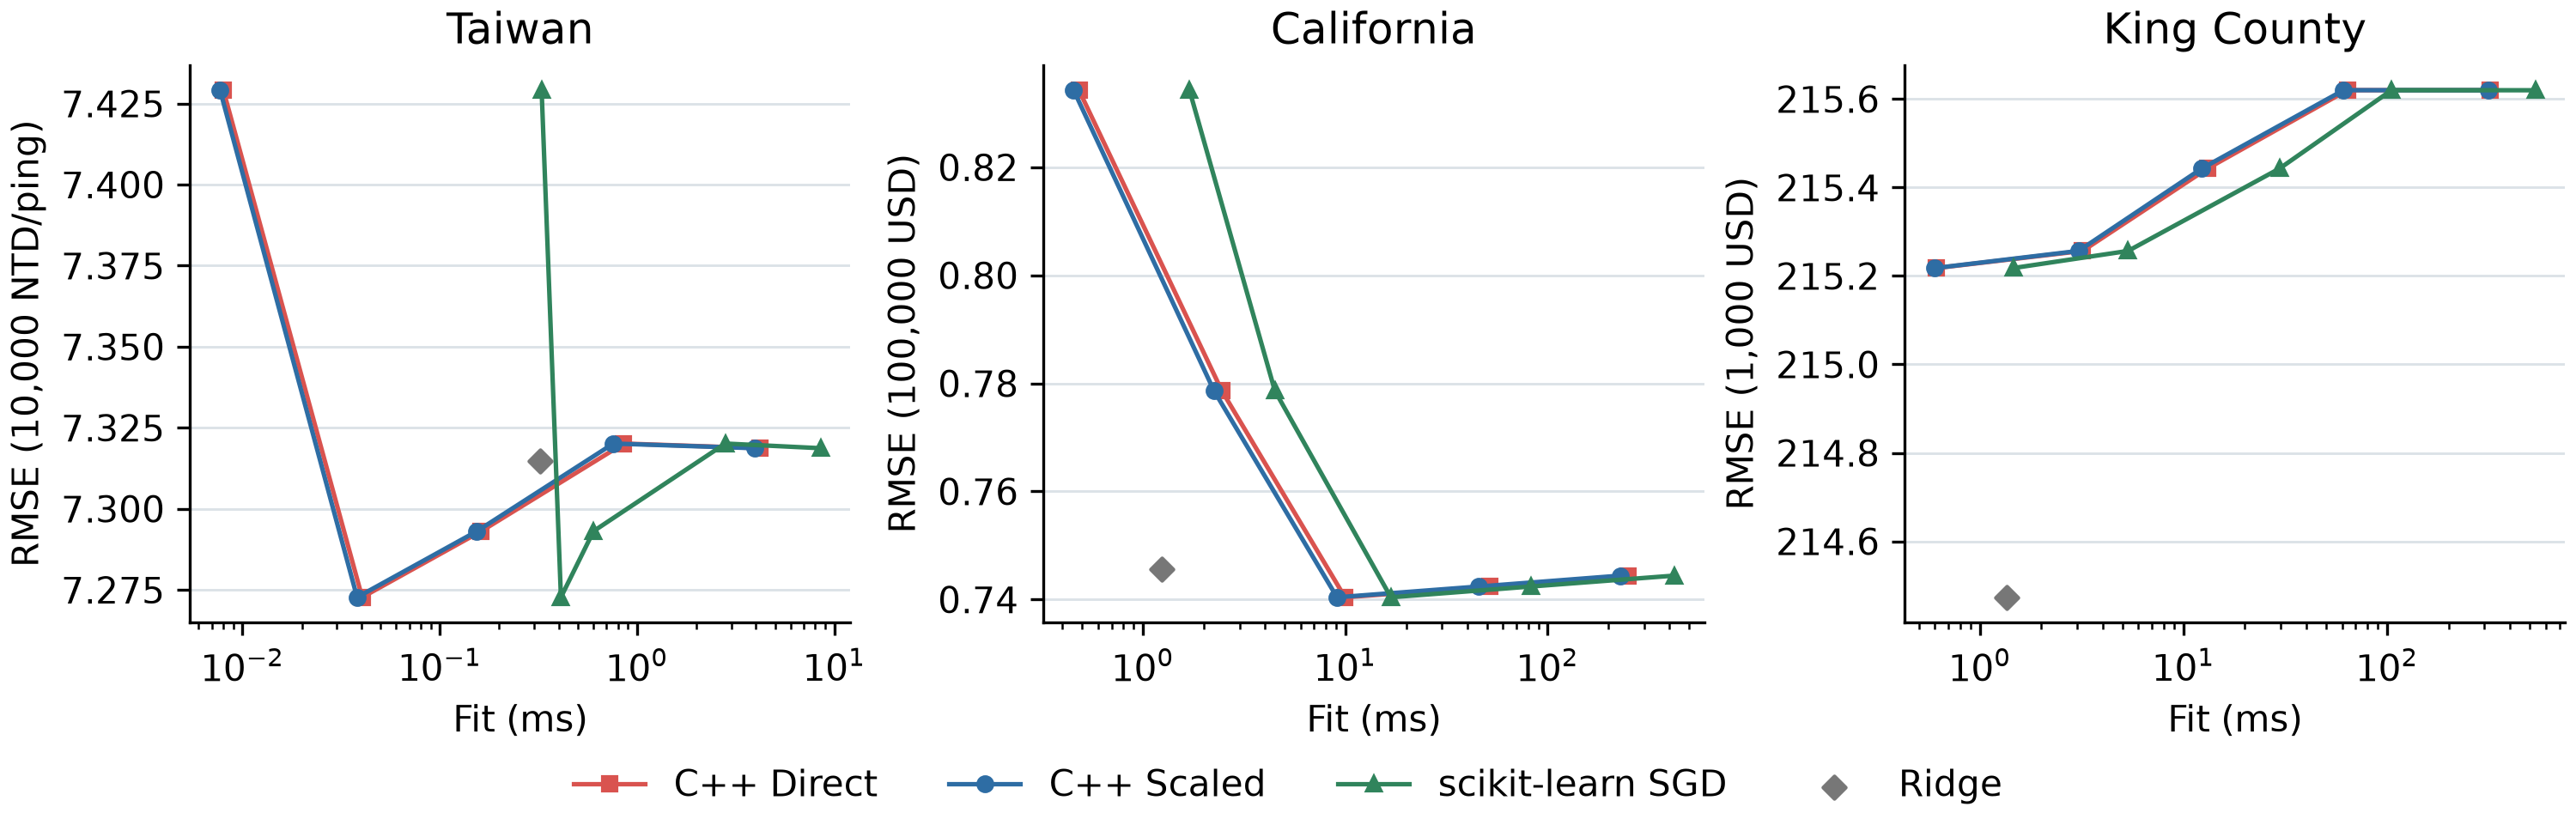
\includegraphics[width=0.94\textwidth]{fig4_rq2_fit_vs_rmse.png}
\caption{Median fit time and test RMSE on the three housing datasets. Each SGD curve connects the measured epoch budgets $E\in\{1,5,20,100,500\}$ in order. Ridge is shown as a separate point.}\label{fig:fit-rmse}
\end{figure*}

\hd{Hypothesis outcomes.} All 7 of 7 hypotheses are supported under the measurement conditions of this report (Table~\ref{tab:hyp}).

\begin{table}[!htb]
\centering\footnotesize
\caption{Verdict on the 7 hypotheses set by us.}\label{tab:hyp}
\begin{tabular}{@{}P{0.85cm}P{4.0cm}P{2.9cm}@{}}
\toprule
ID & Acceptance criterion & Observed\\
\midrule
H1-a & $T_{\mathrm{dir}}/T_{\mathrm{sc}}\ge2$ at $n\ge10^4$, monotonically increasing & $58.65\x$; $600.71\x$; $3197.90\x$\\
H1-b & $\beta_{\mathrm{dir}}\in[0.7,1.1]$, $\beta_{\mathrm{sc}}\le0.35$ & 1.002; 0.133\\
H1-c & $0.5\le T_{\mathrm{dir}}/T_{\mathrm{sc}}\le3$ at 100\% & $1.12\x$\\
H1-d & $\max/\min$ of $T_{\mathrm{sc}}\le1.30$ (Grid C) & 1.11\\
H1-e & $\|w_{\mathrm{sc}}-w_{\mathrm{dir}}\|/\|w_{\mathrm{sc}}\|<10^{-10}$ & $\le5.11\x10^{-14}$\\
H2-a & $\relW<10^{-10}$, $\relR<10^{-6}$ & Direct and Scaled: 15/15 each\\
H2-b & $|d_{\mathrm{cpp}}-d_{\mathrm{sk}}|/d_{\mathrm{sk}}<10^{-6}$ & 0.00\\
\bottomrule
\end{tabular}
\end{table}

\hd{Discussion.} Direct must read and write the whole of $v$ (8 MB when $n=10^6$) for every sample, whereas Scaled touches only $k=20$ entries. The cost therefore no longer scales with $n$, consistent with the slope of 0.133, and most of the gain probably comes from reducing the amount of memory accessed rather than only from reducing the number of arithmetic operations. The benefit is clear when $\rho\lesssim1\%$ ($\ge19\x$) and drops sharply around $\rho\approx10\%$ ($2.95\x$). Near 100\% density, access through column indices may remove the SIMD vectorization available to dense arrays (a conjecture, not measured), so for fully dense data other approaches, such as mini-batch updates with BLAS, should be used. In practice, a cost of about $0.0688\mus$ per sample corresponds to about 14.5 million samples per second on a single CPU thread at $n=10^6$, $k=20$, the same order as the throughput required by high-rate sparse data streams (such as CTR prediction or spam filtering). The C++ version does not need Python; its potential for embedded devices remains to be verified and was not measured here.

% =====================================================================
\section{Conclusion and Limitations}
This paper verifies the $w=s\cdot v$ technique for $L_2$-regularized least-squares regression with an independent C++17 implementation. For RQ1, at $n=10^6$, $k=20$, the scaled loop is about $3198\x$ faster ($0.0688$ versus $219.91\mus$ per step), with the same test RMSE to the reported precision. Its log-log slope is 0.133 (Scaled) versus 1.002 (Direct), consistent with $O(k)$ and $O(n)$. The measured cost varies by a factor of 1.11 across sample counts, and the speed-up narrows to $1.12\x$ at 100\% density. For RQ2, Direct and Scaled meet the equivalence thresholds against \sk{} for all 15 dataset and epoch combinations. The SGD weights approach Ridge ($\dridge$ is 0.7\%--5\% after 500 epochs), while the best observed test RMSE depends on the dataset and epoch budget.

These conclusions should be read within the scope of the experiments:

\hd{Measurement environment.} All measurements were taken on one machine, one compiler (GCC 14.2.0, \texttt{-O2}) and one operating system (Windows 11, which has no standard \texttt{taskset}, so the process could not be pinned to a single core; the spread remains considerable at high density). Absolute times will differ on other machines, and the slight rise at $n=10^6$ depends on the cache size. The relative speed-up and the log-log slopes are properties of the algorithm and are likely to hold, but have not been verified on other architectures. The ``bit-for-bit'' claim also applies only to this environment (same compiler, optimization flags and library versions).

\hd{Data.} The RQ1 data have uniformly random sparsity, whereas real data (TF-IDF, Bag-of-Words) usually follow a Zipf distribution~\cite{zipf}, which can change the cache access pattern even though the per-step complexity $O(k)$ is unchanged. The RQ2 data are small and dense ($n\in\{6,8,17\}$), so they characterize equivalence, convergence and fit time for low-dimensional data.

\hd{Timing scope.} The C++ fit uses CSR, while the scikit-learn fit for housing uses dense input and includes API validation. Prediction timing characterizes the common Python computation used for these experiments. A standalone C++ prediction program has a different measurement scope.

\hd{Algorithmic scope.} Only sequential single-threaded SGD is considered (Hogwild!~\cite{hogwild} is not covered), without early stopping, and with the \texttt{invscaling} schedule on standardized data. The \texttt{optimal} schedule and the forced-reset configuration were used only in unit tests.

Future work is to measure on real sparse data with a Zipf distribution (for example MovieLens or text classification), to try more architectures and compilers, and to extend the study to other loss functions.

% =====================================================================
\section*{AI Usage Declaration}
The initial implementation and write-up used two generative AI tools. \textbf{Gemini 3.8 Flash} (Agent Mode in the Antigravity IDE) assisted with programming: the C++17 code skeleton (\texttt{sgd\_direct.hpp}, \texttt{sgd\_scaled.hpp}, \texttt{csr.hpp}, \texttt{timer.hpp}), the Python scripts (\texttt{gen\_rq1.py}, \texttt{prep\_rq2.py}, \texttt{binio.py}, \texttt{bench\_sklearn.py}), the 38 \texttt{pytest} tests, the \texttt{Makefile} and table export. \textbf{Claude Sonnet 5.5} (Anthropic, free web plan) assisted with writing: section layout, editing and condensing the prose, and standardizing terminology. Codex assisted with the paired benchmark, running and checking the measurements, and updating the English LaTeX paper.
The author takes full responsibility for the content, mathematical correctness, data and conclusions; AI is not a co-author. The original code, formulas and procedures proposed by AI were checked by the author: auditing scikit-learn's Cython code (\texttt{docs/sklearn\_source\_audit.md}), compiling and running everything locally (binary data checked by SHA-256), and verifying the mathematical derivations.

% =====================================================================
% References are ordered by first appearance in the text.
\begin{thebibliography}{99}\footnotesize
\setlength{\itemsep}{1pt}
\bibitem{salton} G. Salton and C. Buckley, ``Term-weighting approaches in automatic text retrieval,'' \emph{Information Processing \& Management}, vol.~24, no.~5, pp.~513--523, 1988.
\bibitem{robbins} H. Robbins and S. Monro, ``A stochastic approximation method,'' \emph{The Annals of Mathematical Statistics}, vol.~22, no.~3, pp.~400--407, 1951.
\bibitem{hoerl} A. E. Hoerl and R. W. Kennard, ``Ridge regression: Biased estimation for nonorthogonal problems,'' \emph{Technometrics}, vol.~12, no.~1, pp.~55--67, 1970.
\bibitem{pegasos} S. Shalev-Shwartz, Y. Singer, N. Srebro and A. Cotter, ``Pegasos: Primal estimated sub-gradient solver for SVM,'' \emph{Mathematical Programming}, vol.~127, no.~1, pp.~3--30, 2011.
\bibitem{bottou} L. Bottou, ``Stochastic gradient descent tricks,'' in \emph{Neural Networks: Tricks of the Trade}, 2nd ed., Springer LNCS 7700, pp.~421--436, 2012.
\bibitem{sklearn} F. Pedregosa \emph{et al.}, ``Scikit-learn: Machine learning in Python,'' \emph{Journal of Machine Learning Research}, vol.~12, pp.~2825--2830, 2011.
\bibitem{yeh} I.-C. Yeh and T.-K. Hsu, ``Building real estate valuation models with comparative approach through case-based reasoning,'' \emph{Applied Soft Computing}, vol.~65, pp.~260--271, 2018.
\bibitem{pace} R. K. Pace and R. Barry, ``Sparse spatial autoregressions,'' \emph{Statistics \& Probability Letters}, vol.~33, no.~3, pp.~291--297, 1997.
\bibitem{openml} J. Vanschoren, J. N. van Rijn, B. Bischl and L. Torgo, ``OpenML: Networked science in machine learning,'' \emph{ACM SIGKDD Explorations Newsletter}, vol.~15, no.~2, pp.~49--60, 2014.
\bibitem{zipf} G. K. Zipf, \emph{Human Behavior and the Principle of Least Effort}. Cambridge, MA: Addison-Wesley, 1949.
\bibitem{hogwild} F. Niu, B. Recht, C. R\'e and S. J. Wright, ``Hogwild!: A lock-free approach to parallelizing stochastic gradient descent,'' in \emph{Advances in Neural Information Processing Systems 24}, pp.~693--701, 2011.
\end{thebibliography}

% =====================================================================
\clearpage\onecolumn
\appendix
\section*{Appendix: Prediction Quality versus Epochs}
\begin{figure}[!htb]
\centering
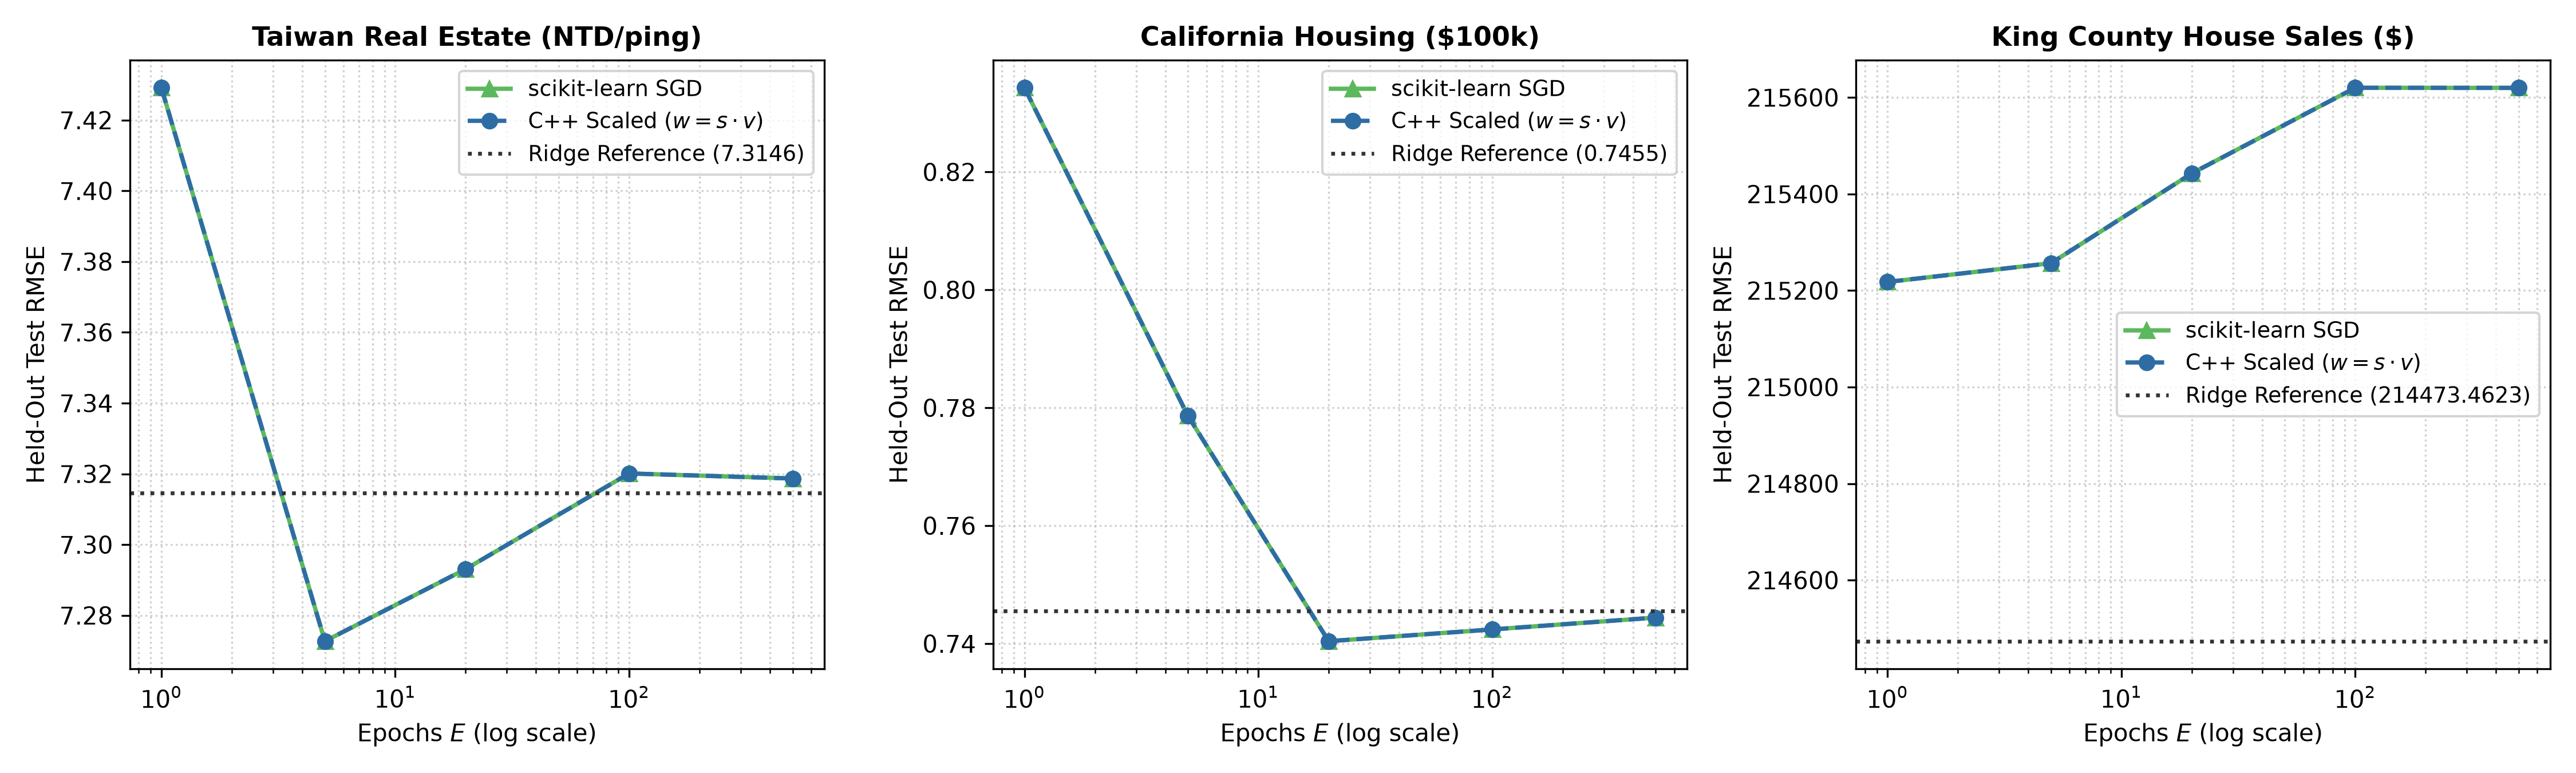
\includegraphics[width=0.95\textwidth]{figS2_rq2_rmse.png}\\[2pt]
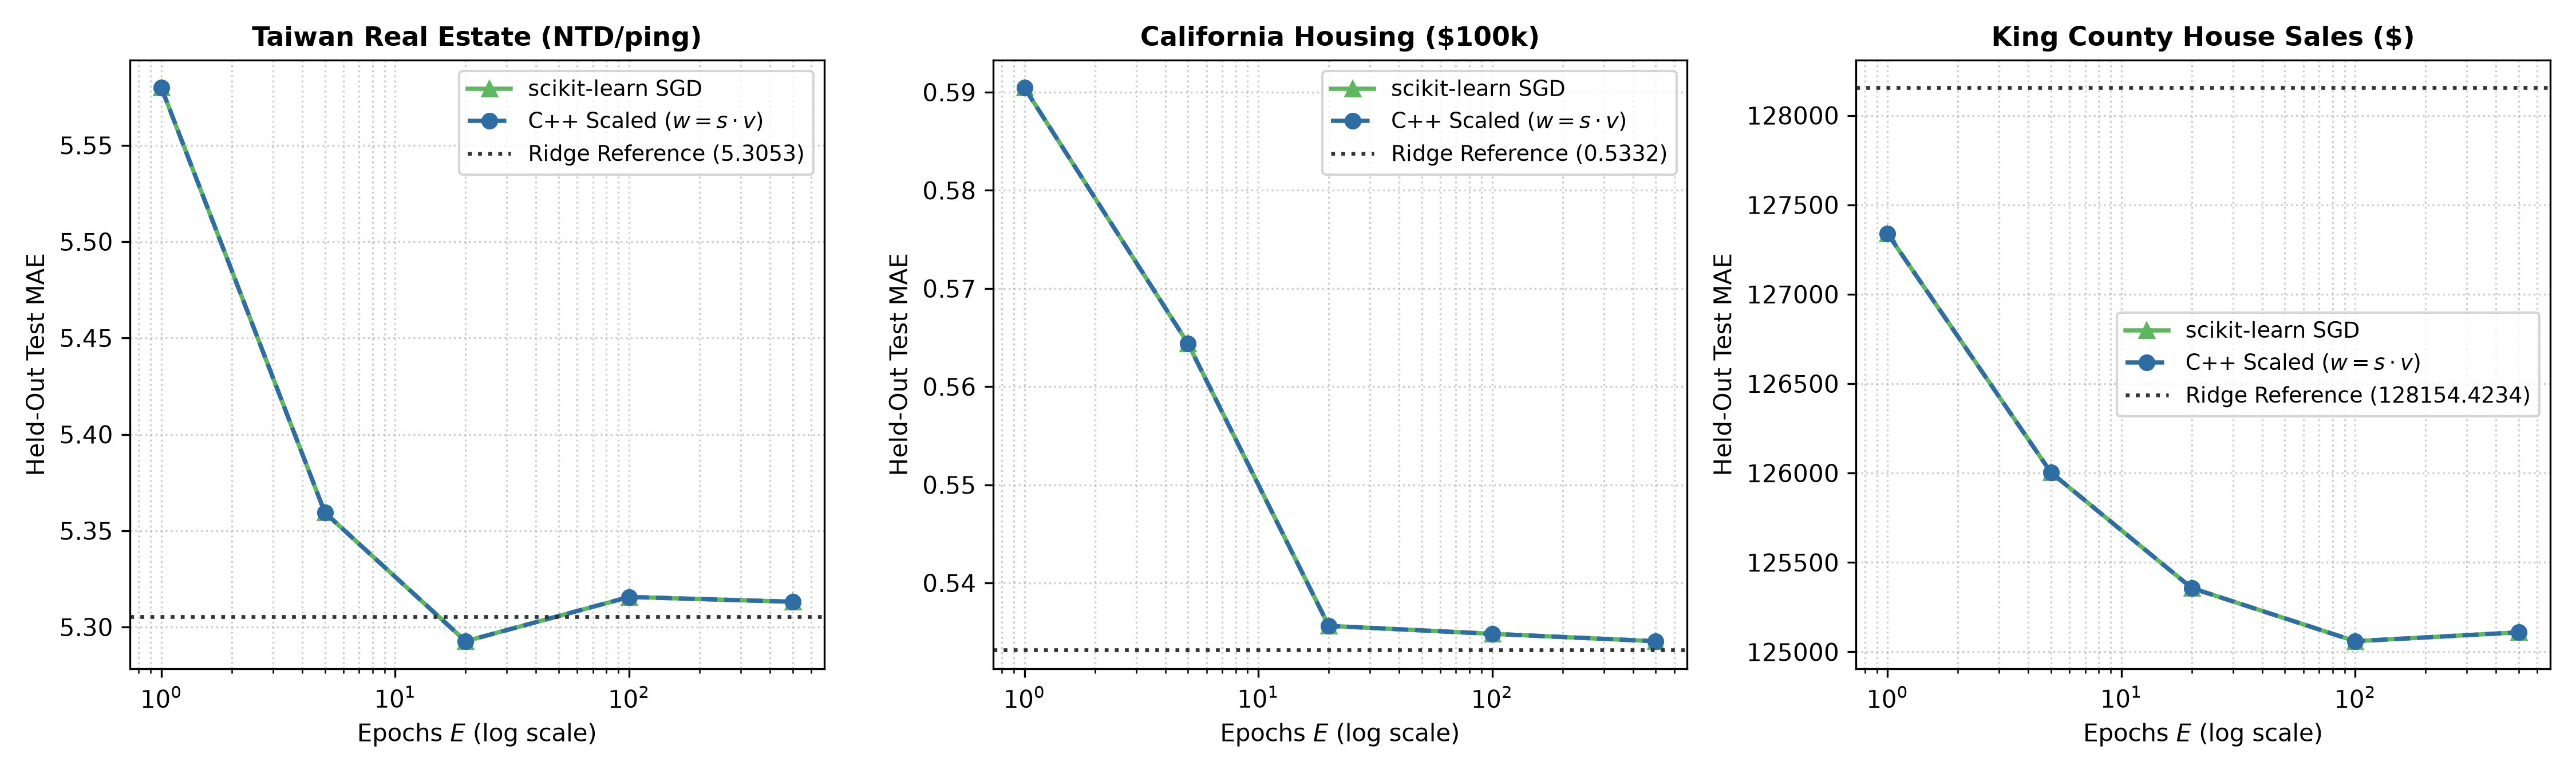
\includegraphics[width=0.95\textwidth]{figS3_rq2_mae.png}\\[2pt]
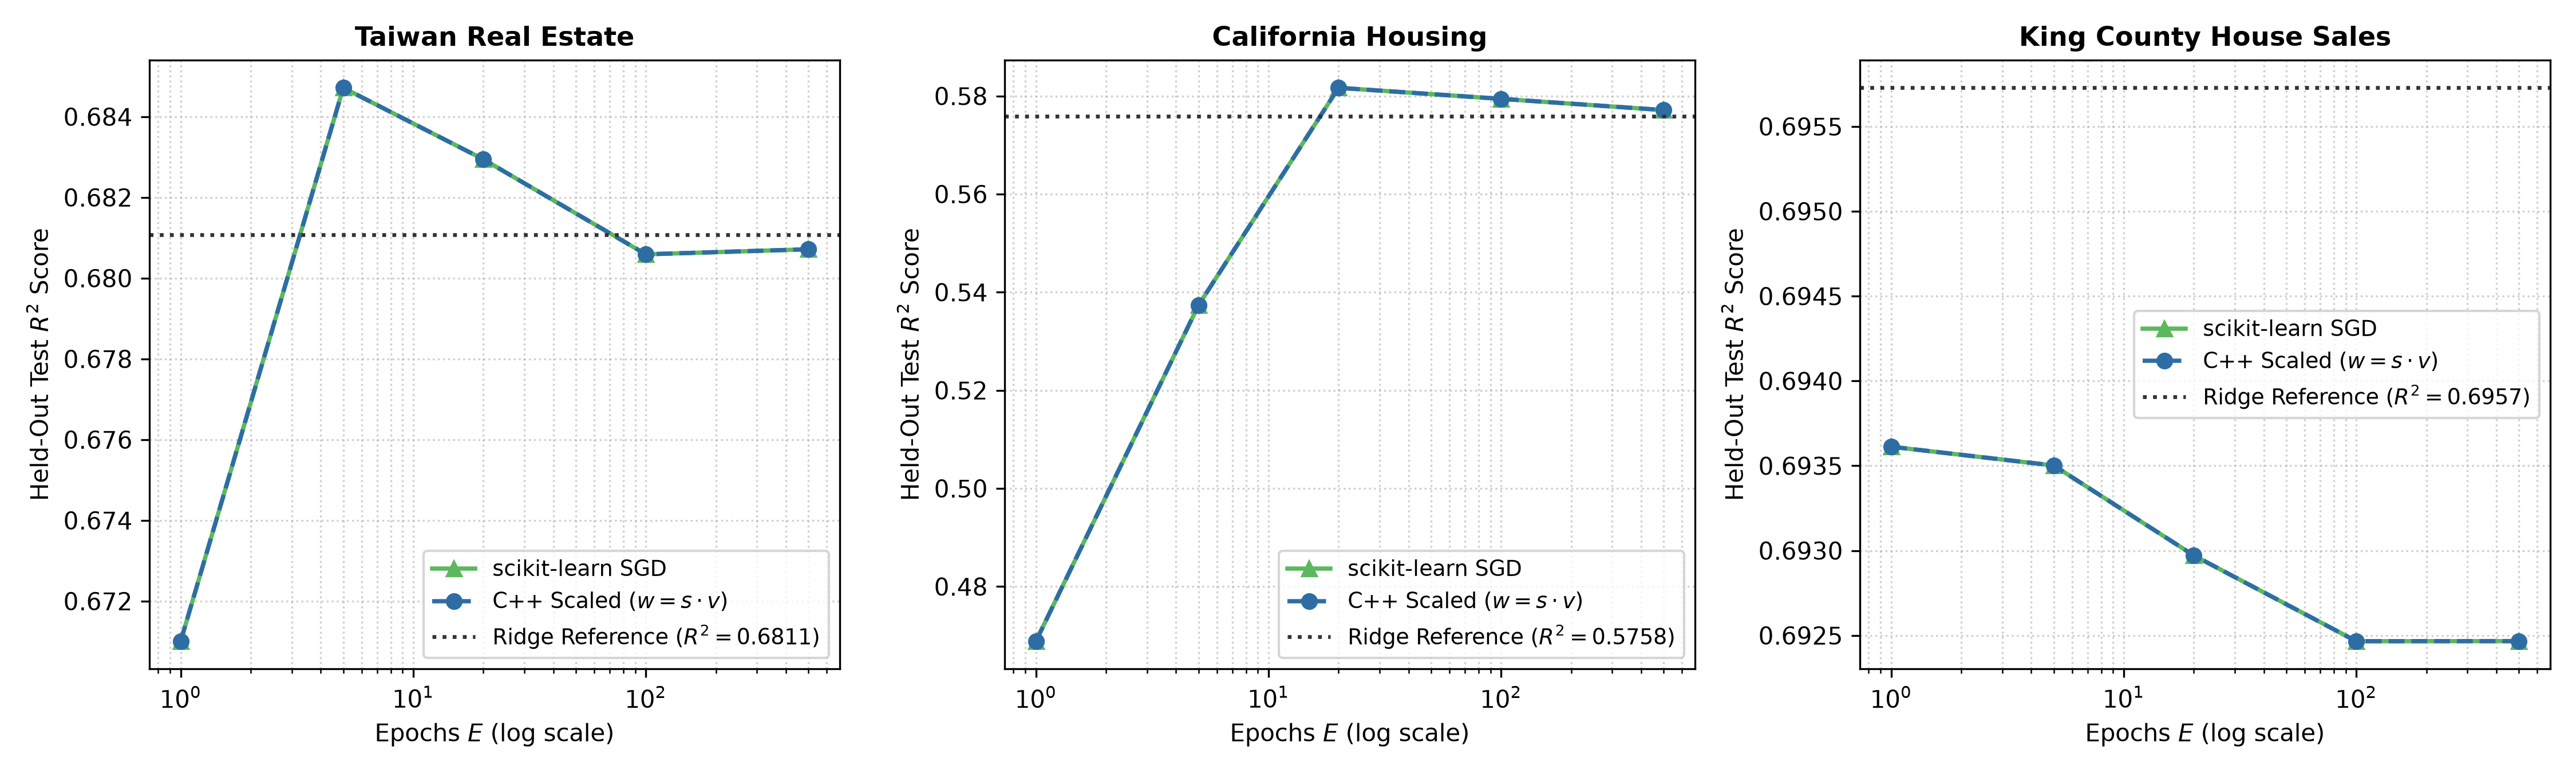
\includegraphics[width=0.95\textwidth]{figS4_rq2_r2.png}
\caption{Test RMSE, MAE and $R^2$ versus number of epochs $E$ (original units). The curves of scikit-learn and C++ Scaled coincide; the dotted line is the Ridge solution.}\label{fig:S}
\end{figure}

\end{document}
